\section{The ASR Problem}
\label{sec:problem}

%\KZ{Here you need to first define what is our input data, that is the
%audio clip. is it mono, or stereo? What is its representation?
%What do we mean by scenes, or context. We need to fix our notation here.
%And then define it as an N-way classification problem just like
%the original ones.}
%\GR{I think it is better to define the input data in evaluation section, because our system can work on both mono and stereo audio. And we need to discuss what is a scene, maybe a synset in wordnet?}
%
The input of the ASR problem is a digital audio clip $A$, and a set of terms $S$
that describe different auditory scenes, such as ``street'', ``supermarket'',
``train station'', etc. The output of the problem is a classification
label $l \in S$ which best characterizes the context or scene
under which $A$ was recorded. This is a typical multi-class classification
problem.

An audio clip in this paper is a single channel, monaural discrete signal
wave such as in \fig{exa}. Stereo sound can be merged into mono sound and
become input to our problem as well.

\begin{figure}[th]
\centering
\epsfig{file=figures/example.eps,width=\columnwidth}
\caption{A waveform of an audio clip recorded in a toilet}
\label{fig:exa}
\end{figure}

Traditional machine learning approach to solving ASR is to first
obtain audio clip samples labeled with scenes from $S$,
and then learn statistical models from audio features extracted from
the training samples. However, because auditory scenes can be complex and
come in large variety, large number of labeled samples are required to train
an accurate model. What's more the clips are required to be long enough to
accommodate sufficient features, hence both the training and storage costs
are high. For uncommon scenes, acceptable training samples are hard to obtain.

Previous research has shown that, human beings recognize auditory scenes
not only by global features but, more critically, by detecting
important events associated with the scene. For the ``toilet'' scene
in \fig{exa}, the distinctive audible events or objects that are
often detected by humans are ``urine'', ``running water'' and ``hand dryer.''
The advantage of recognizing auditory scenes by their constituent events,
is that these basic events usually has shorter durations thus more
training samples available, and are relatively easier to train.
The goal of this paper is to
follow this exact intuition, and infer auditory scenes
without training samples of the scenes. The key challenges would be i)
detecting the sound events from long audio inputs, and ii) relating basic
sound events to the correct scene. We do this by a hybrid technique that
combines text mining with audio signal modeling.

